\section{Proposed Key Recovery Framework}

The proposed framework protects an AES-256 key through threshold sharing while extending the recovery phase with Reed-Solomon-style error correction. The complete workflow has eight stages:
\begin{enumerate}
\item Generate a random AES-256 key.
\item Encrypt the target plaintext with AES-GCM.
\item Convert the AES key to an integer in $\mathbb{F}_{p}$.
\item Split the integer secret into $n$ Shamir shares with threshold $t$.
\item Distribute or store the shares across independent locations.
\item During recovery, collect $m$ available shares.
\item Apply robust reconstruction to tolerate missing or corrupted shares.
\item Use the recovered key to decrypt the ciphertext and verify correctness.
\end{enumerate}

The ordering of these steps matters. The plaintext is encrypted before the key is split so that the recovery procedure handles only a short fixed-size secret rather than an arbitrarily large message. This keeps the secret-sharing layer compact and ensures that the cost of robust reconstruction depends on the key-management problem instead of on the size of the protected data.

Fig.~\ref{fig:workflow} illustrates the end-to-end workflow from AES key generation to robust share-based recovery.

\begin{figure*}[!t]
\centering
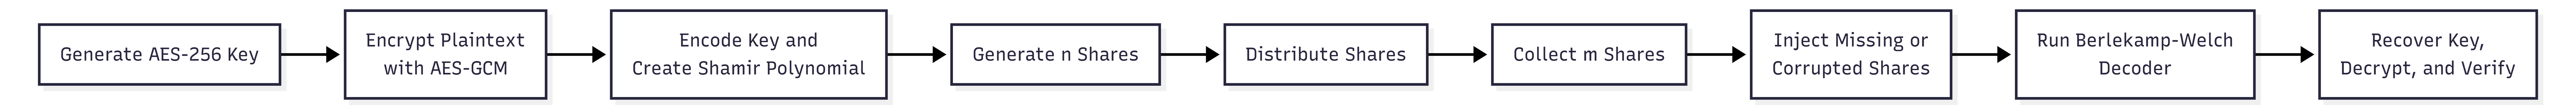
\includegraphics[width=0.96\textwidth,height=2.1in,keepaspectratio,trim=20 20 20 20,clip]{../images/scheme.png}
\caption{End-to-end workflow of the proposed robust AES key recovery framework.}
\label{fig:workflow}
\end{figure*}

Algorithm~\ref{alg:recovery} summarizes the recovery logic. The key observation is that the framework does not replace Shamir's access policy; it refines only the reconstruction stage. If the available shares are all valid, robust recovery reduces to ordinary polynomial interpolation. If a bounded number of shares are corrupted and the redundancy condition in \eqref{eq:bound} holds, the Berlekamp-Welch step recovers the intended polynomial and therefore the original AES key.

\begin{algorithm}[!t]
\caption{Robust AES Key Recovery}
\label{alg:recovery}
\begin{algorithmic}[1]
\Require Threshold $t$, total shares $n$, available shares $\mathcal{S}$, AES-GCM ciphertext package $C$
\Ensure Recovered AES key $K$ or failure
\State Generate a random AES-256 key $K$
\State Encrypt plaintext with AES-GCM under $K$ to obtain $C$
\State Encode $K$ as field element $s \in \mathbb{F}_{p}$
\State Create degree-$(t-1)$ Shamir polynomial $f(x)$ with constant term $s$
\State Distribute $n$ shares $(x_{i}, f(x_{i}))$
\State Collect available shares $\mathcal{S}$ during recovery
\If{$|\mathcal{S}| < t$}
    \State \Return failure
\EndIf
\State Use Berlekamp-Welch decoding on $\mathcal{S}$ to recover $\hat{f}(x)$
\State Extract $\hat{s} = \hat{f}(0)$ and convert it to $\hat{K}$
\State Attempt AES-GCM decryption of $C$ with $\hat{K}$
\If{decryption and authentication succeed}
    \State \Return $\hat{K}$
\Else
    \State \Return failure
\EndIf
\end{algorithmic}
\end{algorithm}

\subsection{Design Assumptions and Parameter Selection}

The framework assumes that the AES key is generated with cryptographically secure randomness and that shares are stored across distinct failure domains. In this setting the threshold $t$ controls the balance between confidentiality and recoverability. A smaller threshold improves availability because fewer shareholders are required during recovery, but it also lowers the number of compromised shares needed for disclosure. A larger threshold has the opposite effect.

The total share count $n$ controls the redundancy budget. When no corruption is expected, the basic reconstruction requirement is only $m \geq t$. When corrupted shares are possible, the choice of $n$ should allow the intended recovery set to satisfy \eqref{eq:bound}. For example, if the design target is to tolerate one corrupted share in a $(3,n)$ system while still recovering from all available shares, then $n$ should be at least $5$. If the target is to tolerate two corrupted shares in a $(5,n)$ system, then at least $9$ shares must participate in reconstruction.

This design targets a specific threat model. It tolerates accidental share loss, partial share compromise below the threshold, and bounded corruption during recovery. It does not claim resistance against an attacker who already possesses at least $t$ valid shares, nor does it protect a workstation that is compromised after the key has been reconstructed.
